\chapter{Testy systemu}
W tym rozdziale przedstawione są różne konfiguracje pakietów, wraz z wykresami ruchów platform, oraz wnioski płynące z tych zachowań.

% \section{Porównanie modeli dynamiki i kinematyki}
% 	Posiadając model kinematyczny, którego ruch jest sterowany wzorami, można porównać jego pozycję i rotację z modelem dynamicznym.
% 	Należy w tym samym momencie nadać bazom identyczne prędkości kół i zebrać dane dotyczące wzajemnej pozycji.
% 	Nadano kołom kolejne prędkości zgodnie z numeracją w rysunku \ref{fig:base_dims}, $[-2 , 1 , 0 , -3]$.
% 	Do zebrania pomiarów posłużył pakiet \texttt{ocznica}.
% 
% 	\begin{figure}[H]
% 	\centering
% 	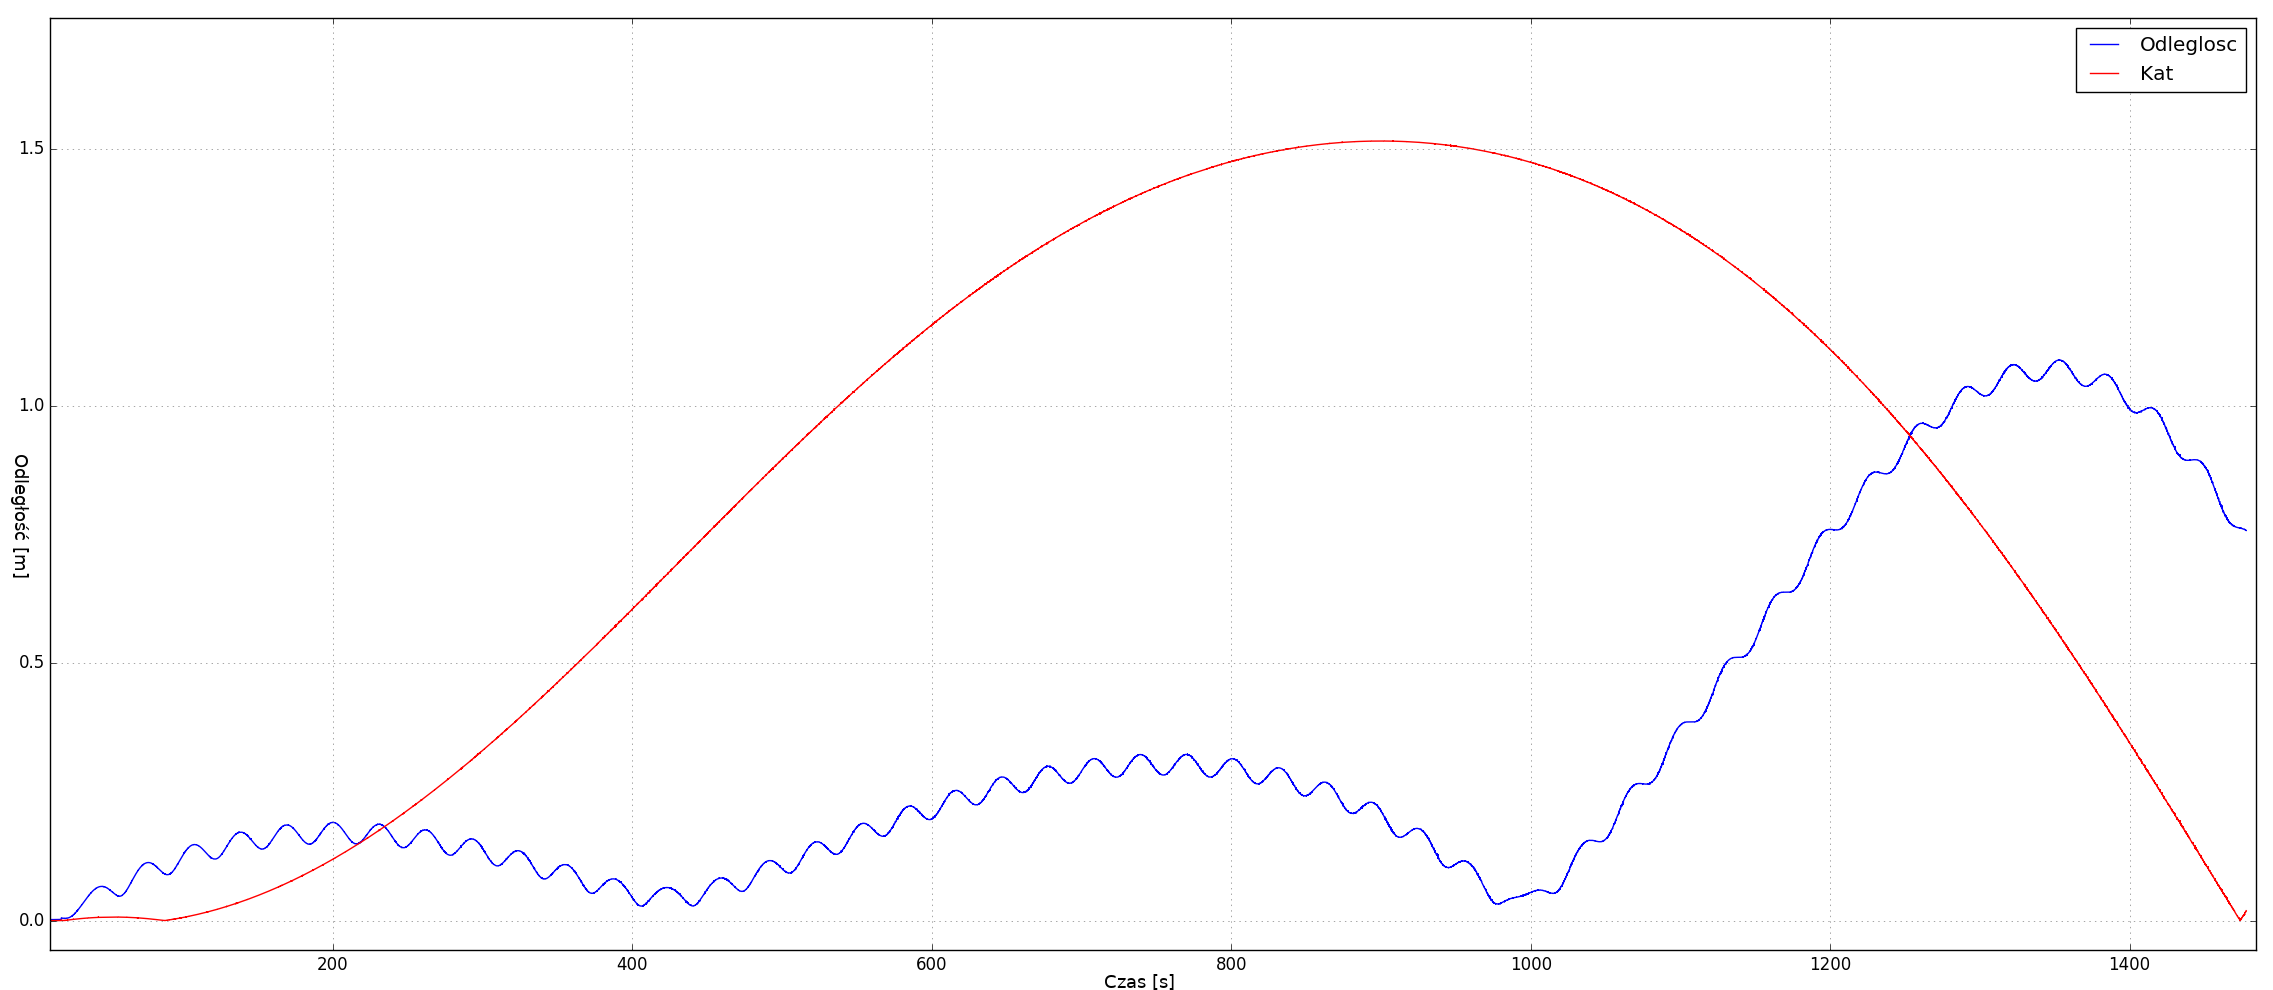
\includegraphics[width=\textwidth]{graphics/test1.png}
% 	\caption{Odległość i kąt pomiędzy platformami w czasie.}
% 	\end{figure} 
% 
% 	%TODO połączenie komponentów na UML, jak nie Tikz to Draw.io
% 	
% 	Takie ustawienie spowodowało ruch po okręgu o okresie ok. 32 s.
% 	Modele początkowo posiadały zbliżoną pozycję i rotację, ale w miarę upływu czasu opóźnienia modelu dynamicznego stały się zauważalne.
% 	Także kąt między nimi zaczął się zmieniać, lecz w znacznie większym stopniu, niż wynikałoby to z opóźnienia pozycji.
% 	Przez cały czas trwania eksperymentu model dynamiczny zrobił kąt pełny w stosunku do kinematycznego, a jego odległość zmieniała się sinusoidalnie.
% 	Oba modele wykonały taką samą ilość obiegów.
% 
% 	Po pierwsze widać, że już na samym początku pomiarów odległość nagle wzrosła, co jest spowodowane poślizgiem platformy przy nadaniu kołom prędkości.
% 	Model kinematyczny rozpoczyna jazdę natychmiastowo.
% 	Dzieje się tak, pomimo doskonałym współczynnikom tarcia, w dodatku masa platformy nie jest dobrana zgodnie z rzeczywistością, a lżejsza.
% 	Ten efekt może być zmniejszony za pomocą ustawiania współczynnika tarcia podłoża, ale nie jest możliwe jego całkowite wyeliminowanie, gdyż jest to cecha maszyn symulacji fizyki.
% 
% 	Drugą zauważalną cechą wykresu są małe oscylacje o okresie jednego obiegu.
% 	Ma to efekt taki sam, jak gdyby obie platformy wystartowały z różnych pozycji, których odległość jest mniejsza od średnicy trasy.
% 	To powodowałby, że odległość między ich pozycjami oscylowałaby w właśnie taki sposób.
% 	Modele wystartowały z tego samego punktu w tym samym czasie, jednakże środek ciężkości modelu dynamicznego nie pokrywał się ze środkiem platformy względem którego obliczano pozycję.
% 	W związku z tym jej ruch odbywa się wokół środka ciężkości masy, ale pozycja jest liczona względem geometrycznego środka.
% 	To pokazuje, że należy bardzo dokładnie ustawić masy elementów składowych w stosunku do rzeczywistego modelu, gdyż w przeciwnym wypadku symulacja obarczona będzie właśnie takimi oscylacjami.
% 	Co więcej, ruchome elementy transportowanego robota manipulującego będą miały wpływ na pozycję środka ciężkości i ruch podstawy.
% 	Dlatego należy wprowadzić element transportowanej masy, którego środek ciężkości powinien być modyfikowalny.
% 
% 	Trzecią cechą są duże oscylacje, rosnące w czasie.
% 	Na razie nie jest dokładnie wiadome, dlaczego powstają.
% 	Warto jednak zauważyć, że nie są zbieżne w czasie z kątem obrotu, gdyż jego wartość ma mniejszy okres.
% 
% 	Opóźnienia powstałe na modelu dynamicznym są cechą dokładności maszyny symulacyjnej fizyki i nie da się ich całkowicie wyeliminować.
% 	Jednakże ich wartość jest znacznie mniejsza od niedokładności wprowadzonej przez niedoskonałość rzeczywistego obiektu.
% 	To oznacza, że model ma rzeczywistą wartość pod kątem pomocy w symulacji robota.


